\documentclass{report}

\usepackage[portuguese]{babel}

\usepackage[letterpaper,top=2cm,bottom=2cm,left=3cm,right=3cm,marginparwidth=1.75cm]{geometry}

% Useful packages
\usepackage{amsmath}
\usepackage{graphicx}
\graphicspath{ {./images/} }
\usepackage[colorlinks=true, allcolors=blue]{hyperref}
\usepackage{etoolbox}
\patchcmd{\abstract}{\null\vfil}{}{}{}

\usepackage{lipsum}


\title{Google TPU}
\author{Fernando Lima, 13672710 \\ Isabella Caselli, 13686685 \\ Rodrigo Michelassi, 13672703}
\date{2024}

\begin{document}
\maketitle
\tableofcontents	% como colocar isso na mesma pagina que o titulo

% --- ABSTRACT --- % 
\begin{abstract}

\setlength{\parskip}{1em}\hspace{0.5cm} Na era do desenvolvimento de sistemas baseados em Inteligência Artificial e redes neurais profundas (Deep Learning), se faz necessário o uso de máquinas super potentes, capazes de processar dados e realizar operações matemáticas de maneira extremamente rápida. Modelos de Machine Learning podem levar horas, até mesmo dias, para serem treinados, devido principalmente a operações como produto interno entre matrizes e a enorme quantidade de dados que são usados, trazendo um prejuízo não apenas de tempo, mas também energético, ambiental e sobretudo lucrativo. 

\hspace{0.5cm} Nesse artigo, iremos tratar brevemente sobre a utilização de Cloud TPUs, unidades de processamento de tensores do Google Cloud, que atuam na otimização do treinamento de modelos de aprendizado de máquina, e que se tornou indispensável na academia e na indústria, para todos estudiosos e profissionais da área.
\end{abstract}

% --- CHAPTER 1 --- % 
\chapter{Introdução}

\setlength{\parskip}{1em}\hspace{0.5cm} A evolução tecnológica tem impulsionado avanços significativos no campo da inteligência artificial, especialmente no desenvolvimento de redes neurais profundas (Deep Learning) e aprendizado de máquina (Machine Learning). Com a crescente complexidade dos modelos e o aumento exponencial na quantidade de dados processados, surgiu a necessidade de hardware especializado, capaz de atender à demanda por poder computacional de maneira eficiente. Nesse contexto, destaca-se a Unidade de Processamento Tensorial (TPU), um circuito integrado de aplicação específica (ASIC) desenvolvido pelo Google para atender às demandas específicas do aprendizado de máquina e inteligência artificial.

Lançadas em 2015, as TPUs foram projetadas para acelerar operações matemáticas essenciais em aprendizado de máquina, como as multiplicações e somas de matrizes, que são fundamentais para o funcionamento de redes neurais. Diferentemente das CPUs e GPUs, cuja arquitetura é generalista e voltada para uma ampla variedade de aplicações, as TPUs possuem uma arquitetura altamente otimizada para tarefas específicas de aprendizado profundo, oferecendo maior eficiência energética e desempenho superior em comparação com soluções tradicionais.

Além de desempenharem um papel crucial no treinamento e na inferência de modelos de aprendizado de máquina, as TPUs também têm permitido avanços significativos em áreas como processamento de linguagem natural, visão computacional e sistemas de recomendação. Sua adoção em larga escala em data centers e projetos de pesquisa reflete a importância desse hardware na computação moderna.

Diante desse cenário, este trabalho tem como objetivo explorar a arquitetura, os princípios de funcionamento e as aplicações das TPUs, destacando sua relevância para os avanços tecnológicos no campo da inteligência artificial e seu impacto na evolução da computação contemporânea.

% --- CHAPTER 2 --- % 
\chapter{História}

\setlength{\parskip}{1em}\hspace{0.5cm} A Google Tensor Processing Unit (TPU) é uma arquitetura de circuito integrado especializada, conhecida como um "acelerador de IA". Essa tecnologia teve sua primeira aplicação em 2015, sendo apresentada ao público em 2016 como uma alternativa inovadora às arquiteturas amplamente utilizadas para acelerar o treinamento de modelos de inteligência artificial, como GPUs e arrays sistólicos.

Embora tenha sido oficialmente divulgada apenas em 2016, engenheiros da Google revelaram que a TPU já era utilizada internamente em data centers da empresa por mais de um ano antes de seu lançamento público. Desenvolvida com foco em desempenho otimizado, a arquitetura foi projetada para integrar-se perfeitamente à biblioteca de aprendizado de máquina TensorFlow, também criada pela Google. O TensorFlow é amplamente utilizado para o treinamento de modelos baseados em redes neurais e, atualmente, figura entre as bibliotecas mais populares e robustas do setor.

Uma das principais funcionalidades das TPUs é o processamento eficiente de tensores, uma estrutura de dados representada como um array multidimensional. Estratégias para multiplicação de tensores, tanto de forma linear quanto paralela, são amplamente estudadas em campos como álgebra linear e computação paralela. As TPUs utilizam conceitos avançados dessas áreas para implementar arquiteturas de processamento de produtos matriciais altamente otimizadas, resultando em um desempenho superior em tarefas específicas de aprendizado profundo.

Atualmente, as TPUs são uma tecnologia proprietária da Google, com acesso restrito principalmente aos serviços da empresa. Usuários podem utilizá-las por meio da plataforma de computação em nuvem da Google ou através do Google Colab, onde é possível acessar versões limitadas ou alugar TPUs mais potentes conforme a necessidade.

% --- CHAPTER 3 --- % 
\section{Aprendizado de Máquina e Redes Neurais}

\setlength{\parskip}{1em}\hspace{0.5cm} Em uma era marcada pela presença de modelos como o ChatGPT, IA generativa, e questões éticas envolvendo o uso de imagens e dados pessoais por grandes empresas, surge a necessidade de compreender o funcionamento dos modelos de aprendizado de máquina. Essa compreensão é fundamental não apenas para o fortalecimento científico, mas também para uma aplicação ética e responsável dessas tecnologias.

O surgimento das TPUs está diretamente associado ao avanço científico e comercial dessas tecnologias, que dependem cada vez mais de grandes volumes de dados para seu treinamento e operação. Esses modelos, ao lidarem com dados em larga escala, exigem imenso poder computacional para processá-los e realizar cálculos matemáticos intensivos, como produtos tensoriais, fundamentais para redes neurais profundas.

De forma resumida, os modelos de aprendizado de máquina consistem na modelagem matemática de problemas com propósitos variados, mas que compartilham um objetivo em comum: permitir que o modelo se ajuste suficientemente bem para fornecer respostas adequadas às entradas recebidas. Em essência, há semelhanças com a computação clássica, onde uma entrada é processada para gerar uma saída correspondente. No entanto, os modelos de aprendizado de máquina possuem uma natureza probabilística, o que significa que não há garantia de que as respostas serão sempre corretas. Ainda assim, são extremamente úteis para resolver problemas difíceis de automatizar.

Por exemplo, para um ser humano, identificar a imagem de um gato é uma tarefa trivial. Contudo, como automatizar tal tarefa? Escrever um algoritmo clássico que reconheça um gato em imagens de diferentes tamanhos, formatos e padrões de cores seria inviável devido à complexidade e variabilidade envolvidas. Nesse cenário, o uso do aprendizado de máquina surge como uma solução poderosa.

Os modelos mais modernos de aprendizado de máquina, em especial aqueles baseados em redes neurais, são construídos a partir de duas etapas principais: o forward propagation e o back-propagation. Redes neurais consistem em nós que representam as features dos dados e pesos atribuídos a cada uma dessas features. O forward propagation envolve realizar produtos vetoriais entre os pesos e os valores dos nós, seguidos por uma função não linear aplicada à soma ponderada das entradas. Já o back-propagation atualiza os pesos com base no erro calculado, utilizando novamente produtos vetoriais para ajustar o modelo.
Essas operações são computacionalmente intensivas, especialmente em redes neurais que podem conter milhares ou até milhões de parâmetros, dependendo de sua complexidade. Para viabilizar tais cálculos, é indispensável utilizar estratégias que combinem paralelismo e algoritmos eficientes, tarefa para a qual as TPUs foram especificamente projetadas. Conforme será abordado adiante, com sua arquitetura otimizada, as TPUs permitem acelerar o treinamento e a inferência de modelos, tornando-os mais acessíveis e práticos no mundo real.

\begin{figure}[h]
	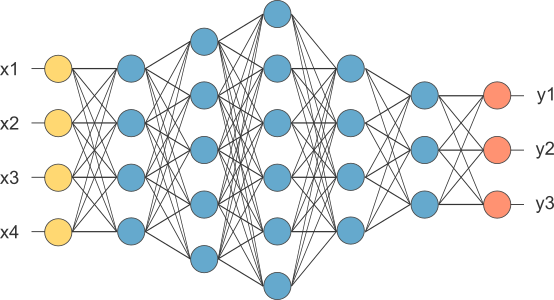
\includegraphics[scale=0.7]{neuralNetwork}
	\centering
	\caption{Estrutura gráfica de uma Rede Neural}
\end{figure}

\setlength{\parskip}{1em}\hspace{0.5cm} Com base nisso, temos um modelo matemático, que atualiza pesos e consegue generalizar saídas para determinadas entradas, porém se ele nem sempre a saída é a esperada, como eles são de fato utilizados? Existem diversas aplicações para esses modelos, e o trabalho de um engenheiro de Machine Learning é treinar um modelo, com dados o suficiente, de forma a minimizar o erro (função de perda) desse modelo, dessa forma aumentando sua acurácia e garantindo que o modelo tenha uma maior probabilidade de acertar as respostas, com base nos dados que são utilizados como entrada. Esse é um clássico problema de otimização. Atualmente, esses modelos tem diversos usos na indústria, como no mercado financeiro, para predição de séries temporais para variações da bolsa de valores, na medicina para auxílio de profissionais no diagnóstico de doenças, no direito para análise textual de casos, na astronomia, como na recente descoberta da primeira imagem de um buraco negro. 

Dessa forma, Machine Learning é uma tendência que cresce tanto no mercado como na academia, e deve continuar sendo explorado por diversos profissionais, de forma que é necessário acelerar o longo processo de treinamento de modelos, além de buscar soluções mais sustentáveis para que o desenvolvimento continue em expansão.

\section{Large Language Models}

\setlength{\parskip}{1em}\hspace{0.5cm} Uma das técnicas mais discutidas atualmente no ramo de Deep Learning é o Processamento de Linguagem Natural (NLP), que ficou ainda mais conhecido quando se tornaram públicos os grandes modelos de linguagem (LLMs). Esses modelos são conhecidos por serem treinados com uma grande quantidade de dados, provindos muitas vezes de toda a internet, como é o caso dos modelos GPT.

Modelos de linguagem no geral são treinados baseados em transfer-learning, ou seja, a utilização de um modelo pré-treinado, onde se ajusta os dados para o modelo desejado, e podem ser utilizados para diversas tarefas, como a criação de chat-bots, agentes inteligentes que interagem com o usuário, automação de tarefas, etc. A ideia geral de LLMs consiste em dar grande poder de generalização para modelos de linguagem, a fim de que o modelo possa realizar "tomadas de decisão" de maneira mais próxima do esperado pelo usuário.

Nesse contexto, sabemos que para um modelo ser capaz de tomar decisões que se possa atender às necessidades de todos os usuários, de modo geral, é necessário, além de ajustes grandes para possíveis respostas (baseados no Attention, que dá maior pesos para tokens mais importantes na saída) um grande número de dados de treinamento, que dizem respeito a grande parte das possíveis entradas de um usuário. Assim, a varredura da internet se torna uma ideia frequente para treinar LLMs, visto que se encontra, atualmente, conteúdos relacionados a maior parte dos assuntos que alguém pode querer fornecer de entrada para um modelo de linguagem.

Tendo isso em vista, como o número de dados para se treinar um modelo de linguagem com forte poder de generalização baseado nas mais diversas entradas possíveis, e atender grande parte das possíveis perguntas de usuários, é necessário um poder computacional enorme para processar os dados e realizar operações lineares, como produto matricial. Assim, TPUs podem ser uma forte alternativa para treinar esses modelos e acelerar esse processo, ao mesmo tempo que economizam energia em relação a arquiteturas mais arcaicas.

% --- CHAPTER 4 --- % 
\chapter{Arquitetura da TPU}

\setlength{\parskip}{1em}\hspace{0.5cm} As TPUs surgem como uma alternativa de arquitetura simples para o usuário, oferecendo uma interface de hardware mais amigável e, ao mesmo tempo, capacidade de processar dados com maior rapidez. Essa eficiência foi essencial para atender às demandas de processamento de redes neurais em 2015. Projetada para operar de forma independente da CPU, a arquitetura da TPU recebe instruções diretamente do servidor ao qual está conectada.

\begin{figure}[h]
	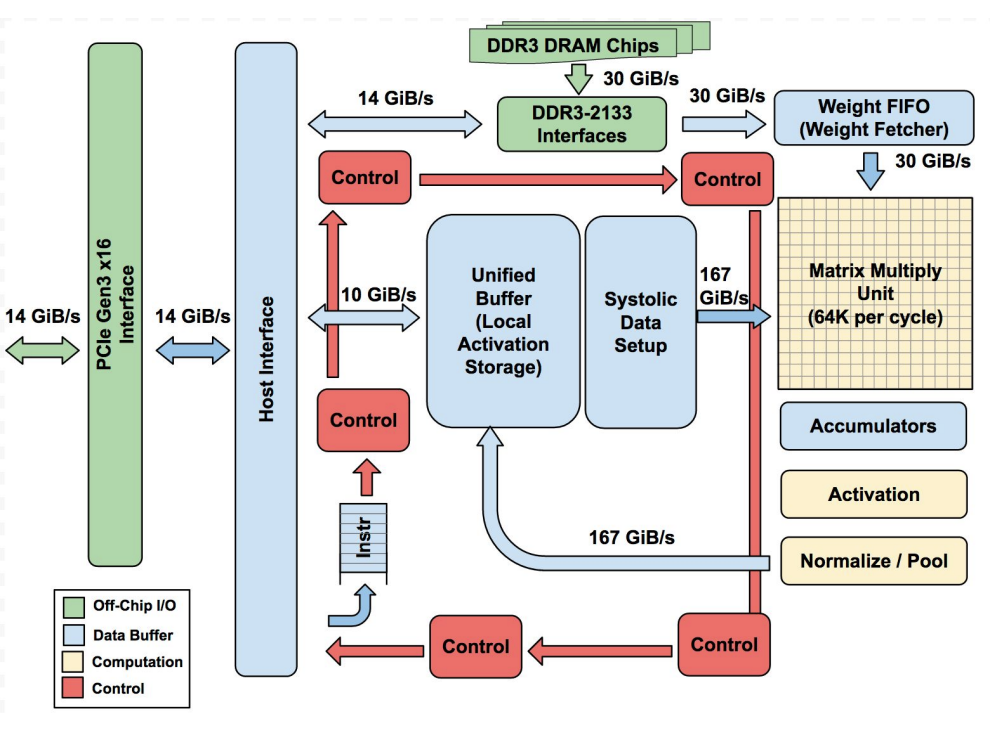
\includegraphics[scale=0.7]{tpu-block-diagram}
	\centering
	\caption{Estrutura básica de uma TPU}
\end{figure}

Para entender melhor a arquitetura de uma TPU, leve em consideração seus pontos mais importantes: a entrada é feita no Weight FIFO, que é levada a principal unidade de processamento, a Matrix Multiply Unit. Essa unidade é responsável por explorar o produto matricial, e iremos explicar mais a fundo em breve. Por fim, a saída é deixada nos acumuladores, e a unidade de ativação performa funções não lineares na saída, para finalmente levar essa saída ao Buffer unificado.

\section{Unidade de Multiplicação Matricial}

\setlength{\parskip}{1em}\hspace{0.5cm} Como dissemos, a unidade de multiplicação matricial é o coração da TPU. Essa unidade contém $256 \times 256$ MACs (endereço de controle de acesso de mídia) que conseguem processar operações de adição de multiplicação em inteiros (com ou sem sinal) de até 8 bits, gerando produtos de até 16 bits, armazenados temporariamente nos acumuladores de 32 bits. Esses acumuladores podem carregar até $4$MiB de dados. A unidade de processamento de matrizes pode computar até $256$ valores por ciclo de clock, e é capaz de realizar operações como produto matricial ou convolução. Vale lembrar que, nos primeiros anos do lançamento da TPU, essa unidade foi planejada justamente para acelerar operações de produto em matrizes densas, sem levar em consideração a esparsidade, que é uma medida útil para acelerar operações de matrizes.

\begin{figure}[h]
	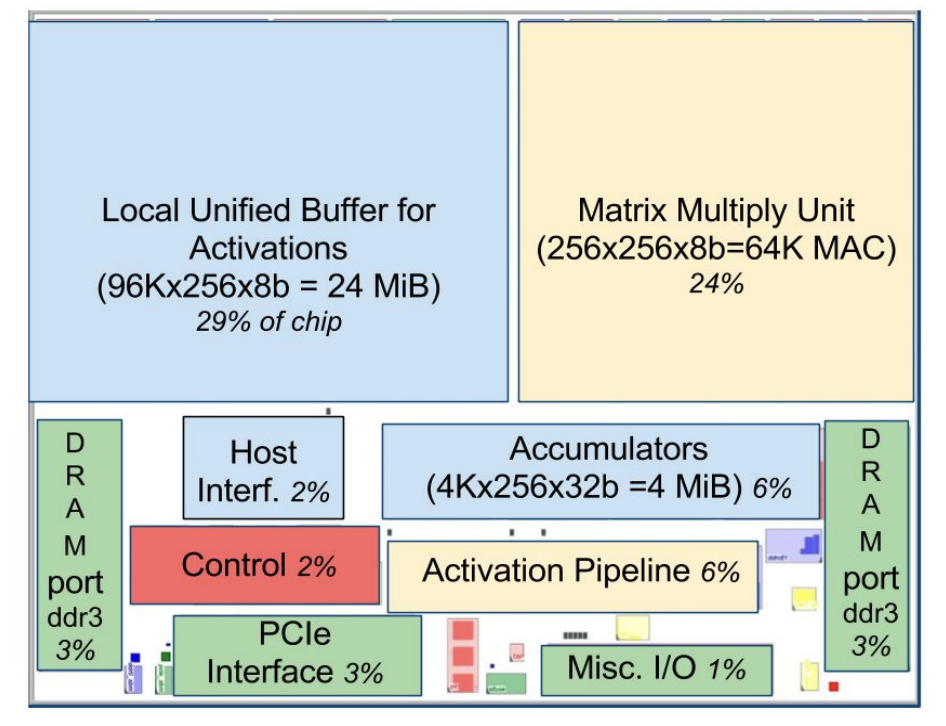
\includegraphics[scale=0.7]{floor-plan}
	\centering
	\caption{Divisão do uso do chip na TPU por unidade}
\end{figure}

Note que, a unidade de processamento de matrizes irá receber muitos dados de entrada, e ler dados da SRAM consome muito mais energia do que processamento aritmético, portanto essa unidade se aproveita de execução sistólica para economizar energia, reduzindo operações de leitura e escrita do Buffer unificado, dependendo de dados provindos de diversas direções alimentando um array em intervalos regulares.

\section{Principais instruções}

\setlength{\parskip}{1em}\hspace{0.5cm} Como vimos, as instruções a serem executadas são enviadas de maneira externa para a TPU, através de PCIe (Peripheral Component Interconnect Express), o que pode ser relativamente lento e caminhar na direção oposta ao que é esperado. Nesse contexto, a fim de acelerar esse processo, a TPU faz uso da arquitetura CISC para definir instruções. A seguir, vemos algumas das principais instruções presentes na TPU:

$\bullet$ Read\_Host\_Memory: lê dados da CPU para o Buffer Unificado da TPU

$\bullet$ Read\_Weights: lê a entrada da unidade matricial

$\bullet$ MatrixMultiply/Convolve: faz com que a unidade matricial performe uma operação de multiplicação ou convolução, e deposite a saída nos acumuladores. Tal operação matricial leva tempo $B \times 256$ da entrada, multiplica por uma constante $256 \times 256$ e produz uma saída de tamanho $B \times 256$, e leva $B$ ciclos de clock para ser concluída.

$\bullet$ Activate: performa a função não linear de ativação no neurônio processado que está no acumulador, podendo ser, nativamente, ReLU, Sigmoid, até mesmo pooling para convoluções. Sua saída é levada para o Buffer unificado.

$\bullet$ Write\_Host\_Memory: escreve os dados do Buffer unificado na CPU.

Como podemos ver, essas principais instruções giram em torno do uso da unidade de processamento de matriz, além de trazer a aplicação de funções conhecidas de Machine Learning, como pooling e funções de ativação, para serem executadas a nível de hardware, acelerando ainda mais o processo. A filosofia geral da TPU é manter a unidade de matrizes sempre ocupada, e processar diversas instruções paralelamente, para evitar que a unidade de matrizes não tenha entrada assim que acabar uma operação.

\section{Compatibilidade}

\setlength{\parskip}{1em}\hspace{0.5cm} Note que a TPU está sendo utilizada sempre de maneira conjunta com a CPU, para recebimento de dados a serem processados. Dessa forma, a pilha de software da TPU tinha como necessidade padrão ser compatível com softwares feitos para rodar na CPU e GPU. Para evitar problemas de compatibilidade, a aplicação de roda na TPU é feita utilizando TensorFlow e compilada em uma API que é capaz de rodar na CPU e GPU.

\begin{figure}[h]
	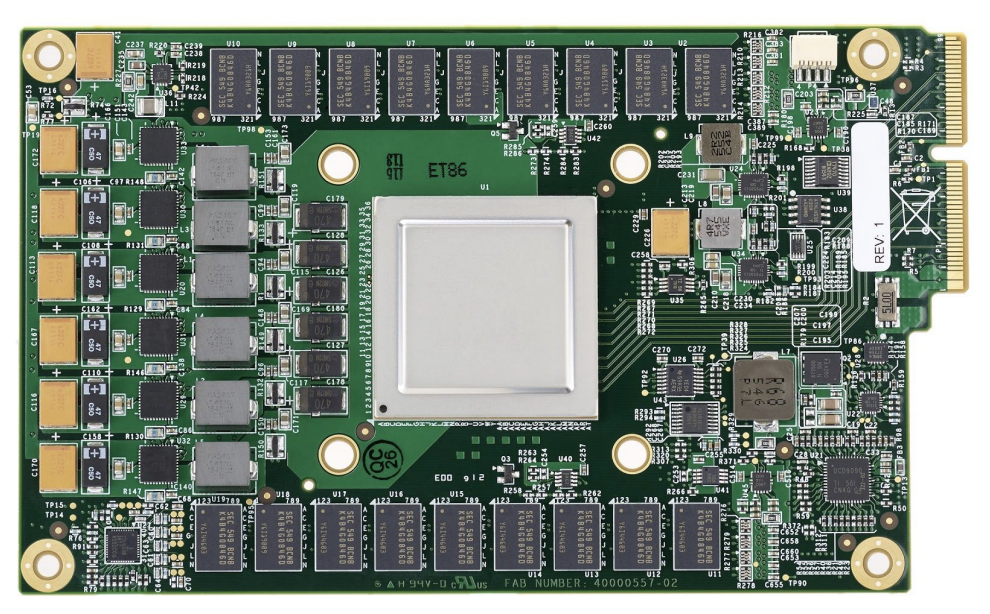
\includegraphics[scale=0.7]{circuit-board}
	\centering
	\caption{Placa de circuito da TPU}
\end{figure}

Atualmente, é possível que usuários possam utilizar gratuitamente a biblioteca TensorFlow, da Google, e rodar seus modelos de aprendizado de máquina utilizando-se da TPU pública presente no Colab, com limite de usos por dia. Para ter acesso a mais seções de uso da TPU ou utilizar arquiteturas mais modernas e poderosas, é necessário assinar um plano da big tech.

% --- CHAPTER 5 --- % 
\chapter{TPU vs GPU}

\setlength{\parskip}{1em}\hspace{0.5cm} As GPUs (Graphics Processing Unit ou Unidade de Processamento Gráfico) são processadores projetados para acelerarem o processamento e a renderização de gráficos e imagens em um computador. Inicialmente, elas foram desenvolvidas para melhorar o desempenho gráfico e aplicações de visualização, mas com o tempo, elas se tornaram ferramentas poderosas também para tarefas de computação paralela. Devido a esta grande vantagem, computar paralelamente, elas tornaram-se vitais nas tarefas de aprendizado de máquina e simulações científicas.

As TPUs e GPUs possuem vantagens distintas e são otimizadas para diferentes propósitos na computação. Embora ambas tenham alguns propósitos em comum, suas arquiteturas e otimizações levam a variações no desempenho, custo e eficiência dependendo da tarefa específica a ser realizada.

\section{Arquitetura e Design}

\setlength{\parskip}{1em}\hspace{0.5cm} A GPU é uma unidade de processamento paralela com milhares de núcleos que podem executar tarefas simultaneamente, acelerando o processo. Sua arquitetura e design são altamente otimizados para executarem cálculos gráficos, por isso ela tem uma capacidade de lidar com enormes quantidades de dados e, devido à sua característica de paralelismo, torna-se adequada para operações matemáticas complexas.

Já as TPUs não possuem tantos núcleos quanto as GPUs, porém, devido à sua arquitetura especializada para o processamento de tensores (operações matriciais), isto permite que elas superem as GPUs em determinadas tarefas. Aprendizagem profunda (Deep Learning), redes neurais, operações de convolução e outras técnicas de aprendizagem de máquina são os principais focos das TPUs.

\section{Desempenho}

\setlength{\parskip}{1em}\hspace{0.5cm} As comparações entre TPUs e GPUs em tarefas semelhantes frequentemente revelam que as TPUs superam as GPUs principalmente em problemas nos quais as TPUs foram especialmente arquitetada para resolver. Logo, as TPUs superam as GPUs em tarefas específicas de aprendizagem profunda, como treinamento extensivo de redes neurais e modelos complexos de machine learning.

Um exemplo seria o treinamento de um modelo ResNet-50 no conjunto de dados CIFAR-10 utilizando uma GPU NVIDIA Tesla V100 leva aproximadamente 40 minutos. Enquanto uma TPU v3 do Google Cloud, o mesmo treinamento leva apenas 15 minutos. Abaixo segue o gráfico deste exemplo.

\begin{figure}[h]
	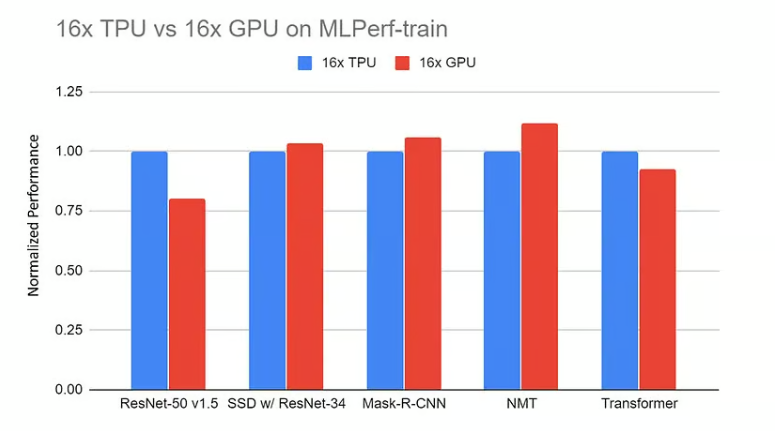
\includegraphics[scale=0.7]{Desempenho}
	\centering
	\caption{Comparação de desempenhos entre TPU e GPU}
\end{figure}


\section{Custos}

\setlength{\parskip}{1em}\hspace{0.5cm} As GPUs possuem um custo relativamente mais acessível em comparação às TPUs, sendo uma das razões para sua popularidade em diferentes aplicações. Um dos principais entraves relacionados às TPUs é o fato de não serem comercializadas individualmente, estando disponíveis exclusivamente por meio de serviços de nuvem. Por outro lado, GPUs podem ser adquiridas diretamente no mercado, com preços que podem alcançar dezenas de milhares de dólares.

Ambas as tecnologias, no entanto, também estão disponíveis por meio de plataformas de computação em nuvem, onde a diferença de custo operacional chama atenção. Por exemplo, o aluguel de uma NVIDIA A100 em serviços de nuvem custa, em média, cerca de 3 dólares por hora. Em contrapartida, o custo para utilizar uma TPU V4 do Google Cloud é significativamente maior, aproximando-se de 8 dólares por hora.

Esta diferença desproporcional está atrelada à grande eficiência das TPUs para tarefas de machine learning em grande escala. Apesar das TPUs terem o custo por hora mais caro, tais tarefas demandam muitas horas de cálculos computacionais. Como existe uma vantagem maior no desempenho das TPUs em relação às GPUs nessas tarefas, o saldo final apresenta-se positivo para a utilização das mesmas.

% --- CHAPTER 6 --- % 
\chapter{Cloud TPU v5p}

\setlength{\parskip}{1em}\hspace{0.5cm} Como discutido anteriormente, os modelos de linguagem de grande escala (LLMs) são atualmente os mais explorados tanto no mercado quanto na academia. Esses modelos dependem de grandes volumes de dados, frequentemente extraídos de vastas partes da internet, cujo crescimento é exponencial. Milhões de novos dados são gerados diariamente, o que torna indispensável que o hardware acompanhe esse crescimento, oferecendo o poder computacional necessário para treinar modelos dessa magnitude.

Diante desse cenário, a evolução das TPUs tem ocorrido de forma acelerada. Em 2023, a Google apresentou a TPU v5p, considerada a mais poderosa já desenvolvida pela empresa. Segundo a Google, o modelo entrega uma performance até 2,8 vezes superior em comparação às gerações anteriores, sendo fundamental para sustentar grandes ecossistemas internos, como YouTube, Android e Gmail.

A TPU v5p se destaca por priorizar o desempenho máximo, mesmo que isso demande maior complexidade operacional. Um dos principais diferenciais dessa arquitetura está na maneira como lida com operações em ponto flutuante. De acordo com dados oficiais, a TPU v5p incorpora 8.960 chips, apresenta três vezes mais memória HBM e atinge uma largura de banda significativamente maior, proporcionando avanços impressionantes na capacidade de processamento.

\begin{figure}[h]
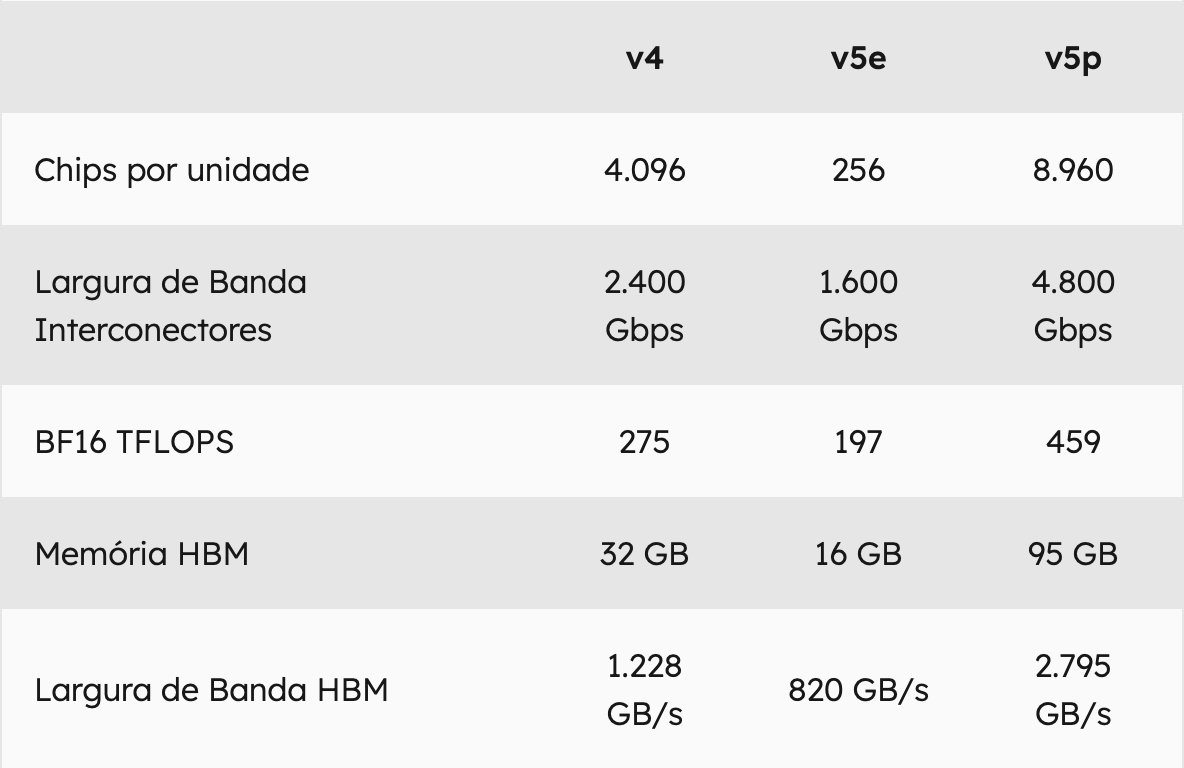
\includegraphics[scale=0.7]{comparativo-tpus}
\centering
\caption{Comparativo entre TPUs Google para cargas de trabalho em IA e LLM}
\end{figure}

Mas o que esses números realmente representam? A Google afirma que a TPU v5p é capaz de escalar o tempo de treinamento de modelos, sendo até 4 vezes mais rápida do que alternativas mais acessíveis, como a TPU v4. Esse aumento de desempenho é atribuído ao dobro da capacidade de operações em ponto flutuante e à maior eficiência proporcionada pela arquitetura revisada.

% --- CHAPTER 7 --- % 
\chapter{Consumo de Energia}

\setlength{\parskip}{1em}\hspace{0.5cm} Atualmente, TPUs são encontradas com maior frequência em data centers, e são um produto extremamente utilizado não só pela Google, como também por empresas e usuários que dependem de seus serviços de nuvem.

Para avaliar, primeiramente, a performance/watt da TPU, e comparar com outras arquiteturas como GPU, se utiliza as métricas "total" (que calcula a energia consumida pela TPU/GPU juntamente a CPU, quando calcula performance/watt) e "incremental" (que subtrai a energia consumida pela CPU). A figura abaixo ilustra bem os resultados obtidos pela Google, que mostram uma performance de $17$ a $34$ vezes melhor que a GPU no modelo total, e de $25$ a $29$ vezes melhor que a GPU no modelo incremental.

\begin{figure}[h]
	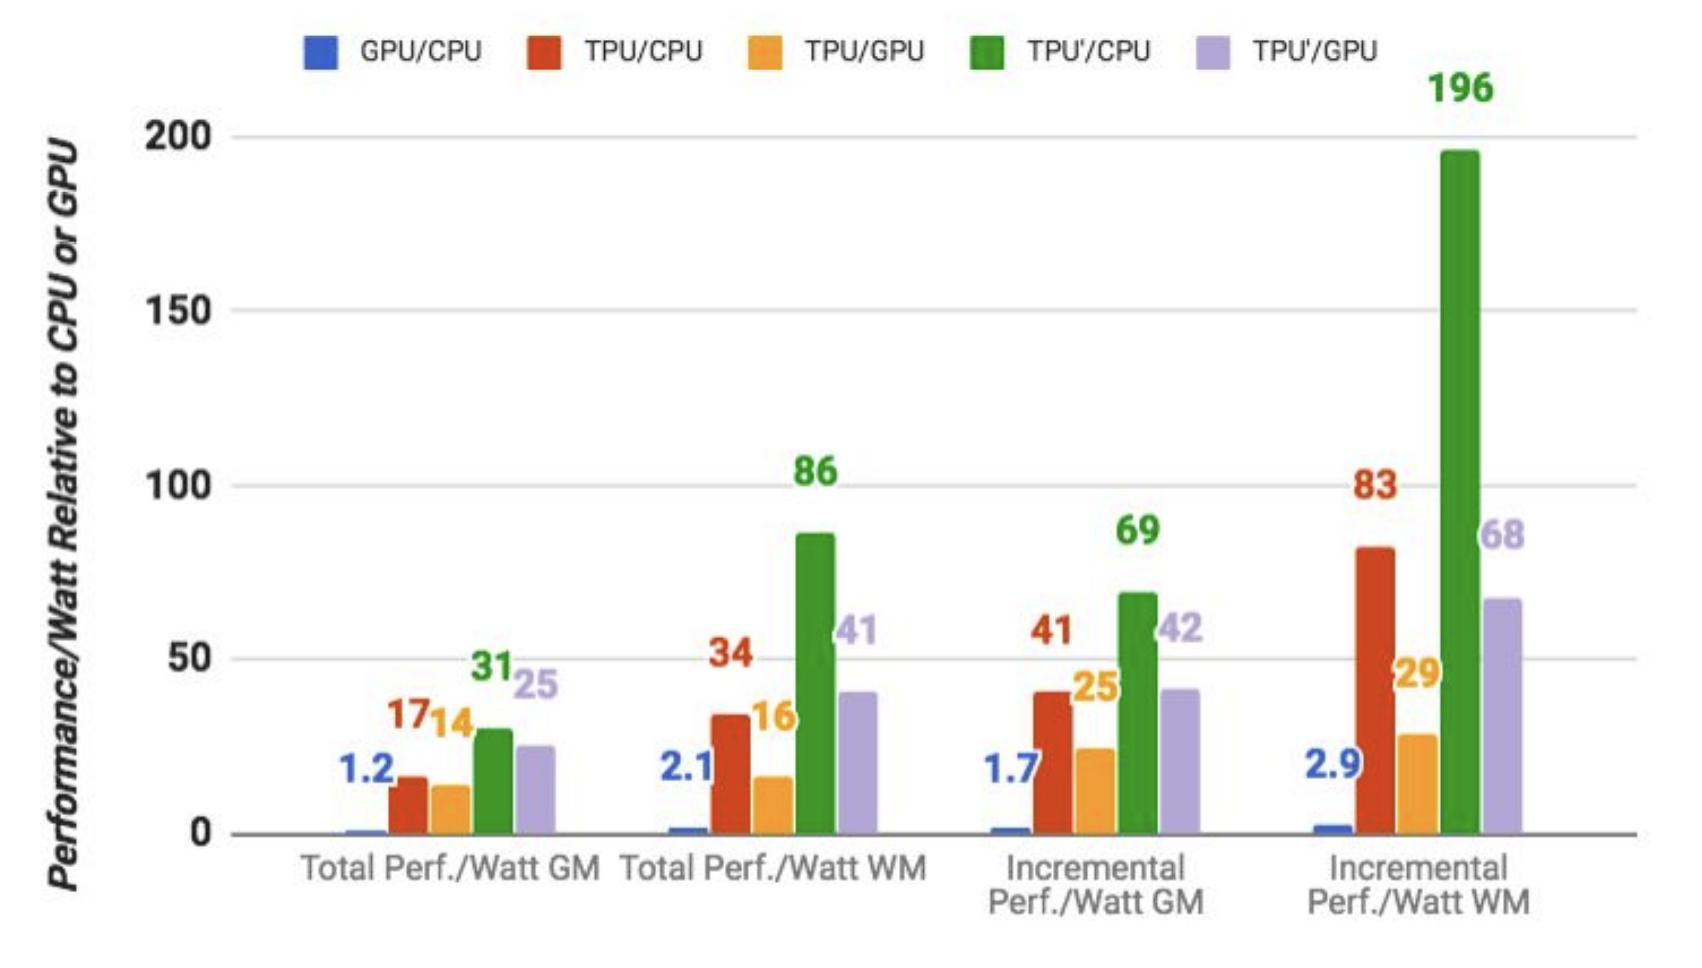
\includegraphics[scale=0.5]{performance-watt}
	\centering
	\caption{Performance/Watt para operações de médias geométricas e ponderadas (GM e WM, respectivamente)}
\end{figure}

Tendo esses consumos em vista, uma das medidas adequadas para se medir, juntamente ao surgimento de uma nova arquitetura, é o TDP (Thermal Design Power), que afeta diretamente o custo de energia gasto, tendo em vista que é necessário que a unidade receba energia e resfriamento suficientes. Assim, dado que servidores não estão em funcionamento durante $100\%$ do tempo, é interessante que a energia consumida por essas máquinas seja proporcional ao seu tempo de uso.

A fim de medir tal consumo e avaliar a validade energética do uso de TPUs em detrimento de GPUs, a figura a seguir compara a energia gasta pelo servidor dividido pelo número de dias, variando o workload para processar CNN0, utilizando o mesmo batch para todos os testes.

\begin{figure}[h]
	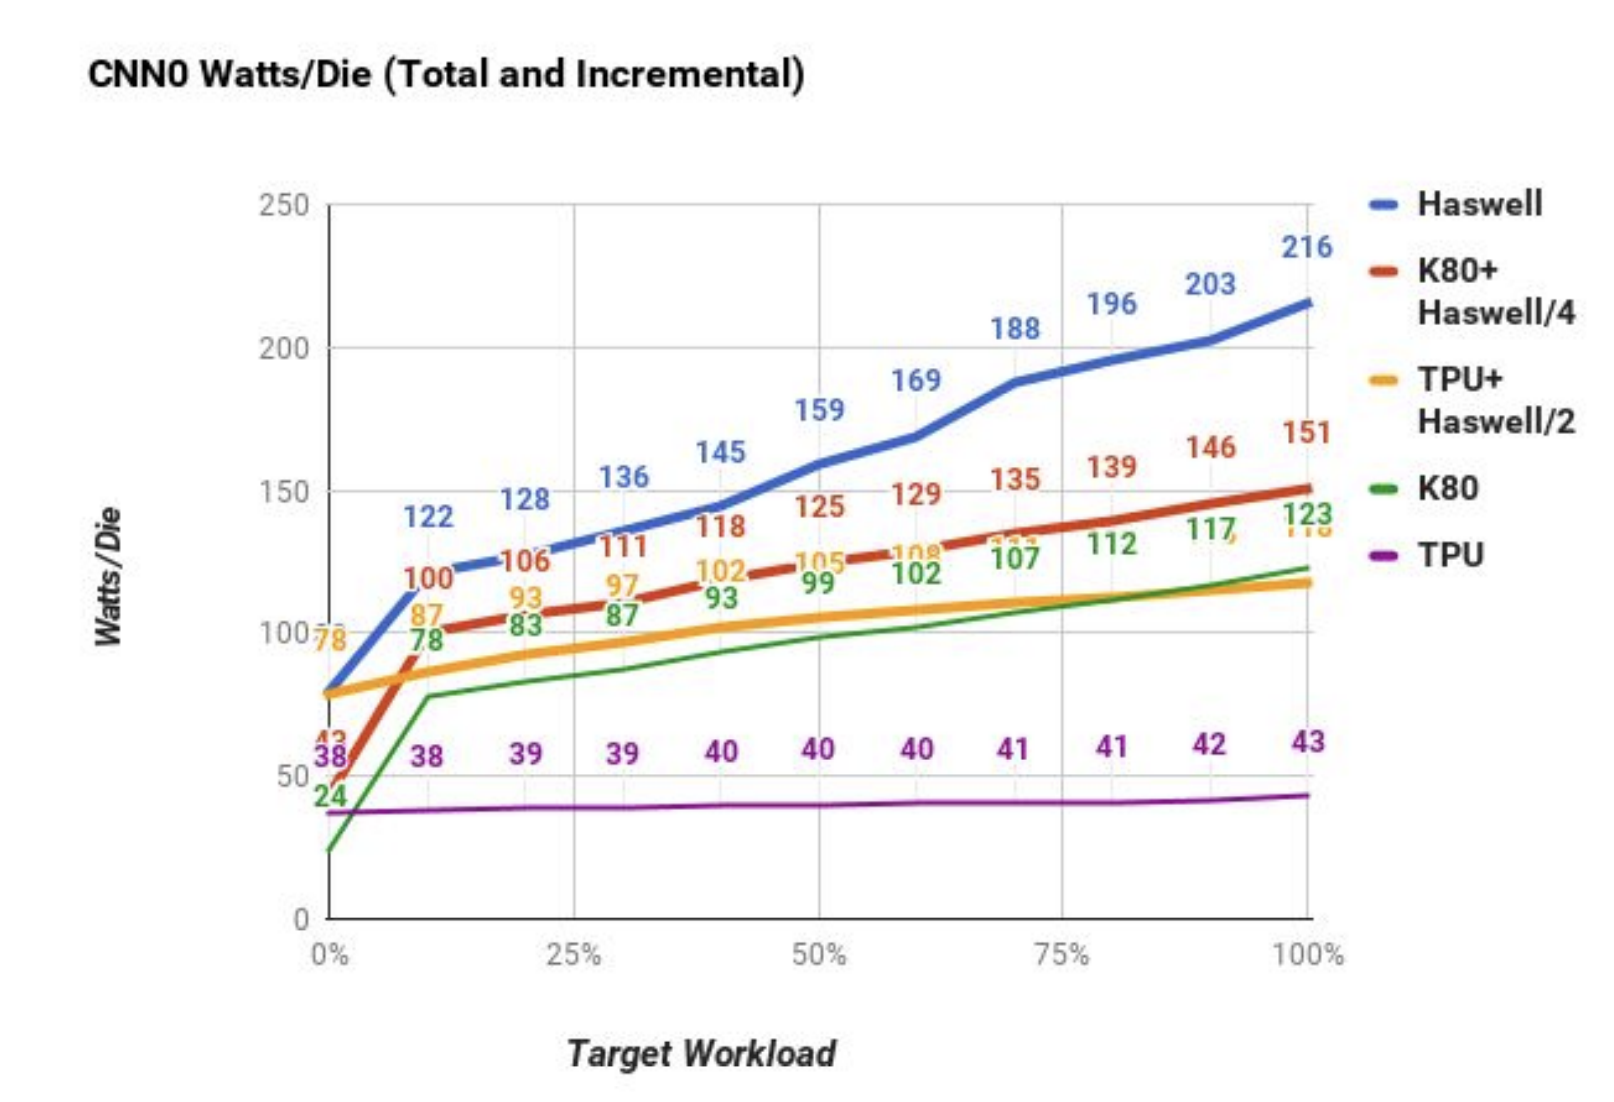
\includegraphics[scale=0.5]{watts-die}
	\centering
	\caption{Performance/Watt para operações de médias geométricas e ponderadas (GM e WM, respectivamente)}
\end{figure}


Pelos resultados obtidos, vemos que as TPUs conseguem consumir, no geral, menos energia que as GPUs. Porém, há um trade-off considerável, pois a quantidade de energia consumida, mesmo com pouca operação na máquina, ainda é muito similar ao consumo com a máquina funcionando em $100\%$. Ou seja, quando a TPU e GPU estão totalmente carregadas, o servidor de CPU gasta $52\%$ da energia da GPU e $69\%$ da energia da TPU. Nesse sentido, a TPU ainda gasta mais energia proporcionalmente, pois realiza muito mais tarefas que a GPU, mas seus gastos em valor absoluto ainda são inferiores, e justificam o uso desse hardware.

% --- CHAPTER 8 --- % 
\chapter{Considerações Finais}

\setlength{\parskip}{1em}\hspace{0.5cm} Considerando os fatores discutidos ao longo desta monografia, observa-se que o avanço constante de técnicas e algoritmos de alto custo computacional exige o desenvolvimento contínuo de ferramentas de hardware com elevado poder de processamento. Esse progresso é essencial para viabilizar o escalonamento de processos e tarefas cada vez mais complexos, atendendo às demandas impostas por algoritmos modernos. Essa necessidade se torna particularmente evidente no contexto do treinamento de modelos de Deep Learning, que dependem intensivamente de operações matriciais e convolucionais, as quais requerem unidades de processamento capazes de executá-las de forma eficiente e veloz.

Nesse cenário, a Google Tensor Processing Unit (TPU) emerge como uma das inovações mais significativas na área de arquitetura de computadores nos últimos anos. Além de sua ampla adoção pela própria Google, as TPUs vêm sendo utilizadas por inúmeros clientes ao redor do mundo, demonstrando seu impacto global. Como discutido, essas unidades de circuito integrado não apenas aceleram o desenvolvimento e treinamento de modelos de aprendizado de máquina, mas também se destacam pelo compromisso com a sustentabilidade, ao reduzirem significativamente o consumo energético em comparação com processadores convencionais, como as GPUs.

Assim, concluímos que, além do ganho de poder computacional, as TPUs são uma ótima alternativa sobre como as futuras tecnologias de processamento de dados em larga escala devem ser projetadas. Além de impulsionarem o desenvolvimento de softwares de alta demanda computacional, elas abrem caminho para soluções mais sustentáveis, contribuindo para um equilíbrio entre eficiência tecnológica e responsabilidade ambiental.

\bibliographystyle{alpha}
\bibliography{sample}

JOUPPI, Norman P.; YOUNG, Cliff; PATIL, Nishant; PATTERSON, David; e outros. In-Datacenter Performance Analysis of a Tensor Processing Unit. Proceedings of the 44th International Symposium on Computer Architecture (ISCA), Toronto, Canadá, jun. 2017. Disponível em: \href{https://arxiv.org/pdf/1704.04760}{https://arxiv.org/pdf/1704.04760}. Acesso em: 10 dez. 2024.

TPU vs GPU for AI: What's the Difference? Disponível em: \href{https://www.datacamp.com/pt/blog/tpu-vs-gpu-ai}{https://www.datacamp.com/pt/blog/tpu-vs-gpu-ai}. Acesso em: 04 dez. 2024.

NAVEED, Humza; KHAN, Asad Ullah; QIU, Shi; SAQIB, Muhammad; ANWAR, Saeed; USMAN, Muhammad; AKHTAR, Naveed; BARNES, Nick; MIAN, Ajmal. A Comprehensive Overview of Large Language Models. Preprint submitted to Elsevier, 17 out. 2024. Disponível em: \href{https://arxiv.org/pdf/2307.06435}{https://arxiv.org/pdf/2307.06435}. Acesso em: 12 dez. 2024.

RUN.AI. Google TPU: Everything You Need to Know. Disponível em: \href{https://www.run.ai/guides/cloud-deep-learning/google-tpu}{https://www.run.ai/guides/cloud-deep-learning/google-tpu}. Acesso em: 04 dez. 2024.

VAHDAT, Amin; LOHMEYER, Mark. Performance per Dollar of GPUs and TPUs for AI Inference. 11 set. 2023. Disponível em: \href{https://cloud.google.com/blog/products/compute/performance-per-dollar-of-gpus-and-tpus-for-ai-inference}{https://cloud.google.com/blog/products/compute/performance-per-dollar-of-gpus-and-tpus-for-ai-inference}. Acesso em: 04 dez. 2024.

TREFILIO, Daniel. Cloud TPU v5p é o novo e mais poderoso acelerador de IA do Google. Editado por Jones Oliveira. 06 dez. 2023. Disponível em: \href{https://canaltech.com.br/inteligencia-artificial/cloud-tpu-v5p-e-o-novo-e-mais-poderoso-acelerador-de-ia-do-google-272299/}{https://canaltech.com.br/inteligencia-artificial/cloud-tpu-v5p-e-o-novo-e-mais-poderoso-acelerador-de-ia-do-google-272299/}. Acesso em: 04 dez. 2024.

Guia de TPU. Disponível em: \href{https://www.tensorflow.org/guide/tpu?hl=pt-br}{https://www.tensorflow.org/guide/tpu?hl=pt-br}. Acesso em: 12 dez. 2024.

Tensor Processing Unit. Disponível em: \href{https://en.wikipedia.org/wiki/Tensor_Processing_Unit}{https://en.wikipedia.org/wiki/Tensor\_Processing\_Unit}. Acesso em: 10 dez. 2024.

\end{document}